\appendix
\chapter*{Appendix}\addcontentsline{toc}{chapter}{Appendix}
\section{EMF Modeling and VIATRA Query}
\label{sect:emf-viatra}
Although EMF is not a graph database, with the help of VIATRA Query, the data stored in an EMF instance model can be queried like graph databases.

\subsection{Modeling}
Modeling is a versatile concept, the word itself may refer to various topics. In the context of this thesis, by models I primarily mean data models. A data model---or sometimes called domain model---organizes the data elements, how they relate to each other and what actions one can perform on them.

\subsubsection{Metamodels and Instance Models}
\textquote[\cite{scm}]{Metamodeling is a methodology for the definition of modeling languages. A metamodel specifies the abstract syntax (structure) of a modeling language. Metamodels are expressed using a metamodeling language that itself is a modeling language. The metamodel can also be interpreted as the object-oriented data model of the language under design. Metamodeling can be viewed as the grammar for a \emph{typed property graph}, so the created models are both \emph{typed graph}s and \emph{property graph}s.}

The metamodel contains the main concepts and relations of the domain specific language (DSL) and defines the possible structure of the instance models. To enrich the expressive power of the language, attributes are added to the concepts. By doing this, the language can be extended with predefined domains of data types (like integers, strings) that are supported by the metamodeling language. Additionally, some structural constraints might be specified with the elements like multiplicity.

Models describing a particular problem in the domain, called instance models, are defined using the elements of the metamodel.

\subsection{The Eclipse Modeling Framework}
\label{sect:emf}
Eclipse is a free, open-source software development environment and a platform with extensible plug-in system for customization. Eclipse comes with its own modeling tools, with the core framework called Eclipse Modeling Framework (EMF).

\textquote[\cite{EMF}]{The EMF project is a modeling framework and code generation facility for building tools and other applications based on a structured data model. From a model specification described in XMI, EMF provides tools and runtime support to produce a set of Java classes for the model, along with a set of adapter classes that enable viewing and command-based editing of the model, and a basic editor. EMF (core) is a common standard for data models, many technologies and frameworks are based on.}

\subsubsection{Ecore}
Ecore is the metamodeling language used by EMF. It has been developed in order to provide an approach for metamodel definition that supports the direct implementation of models using a programming language. Ecore is the de facto standard metamodeling environment of the industry, and several domain-specific languages are defined using this formalism.~\cite{scm}

\begin{figure}[!ht]
	\centering
	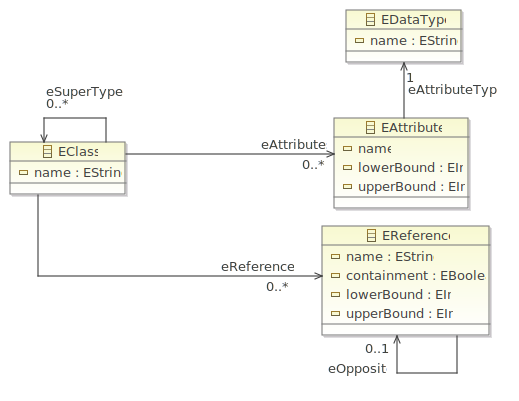
\includegraphics[height=10cm]{include/figures/Ecore}
	\caption{An illustrative core part of Ecore, the metamodeling language of EMF}
	\label{fig:Ecore}
\end{figure}

\Cref{fig:Ecore} shows only a small fraction of the metamodel, as there is many more classes in the Ecore metamodel. The main classes are the following:
\begin{itemize}[topsep=0pt]
	\item \code{EAttribute} represents a named attribute literal, which also has a type.
	\item \code{EClass} represents a class, with optional attributes and optional references. To support inheritance, a class can refer to a number of supertype classes.
	\item \code{EDataType} is used to represent simple data types that are treated as atomic (their internal structure is not modeled). Data types are identified by their name.
	\item \code{EReference} represents a unidirectional association between \code{EClass}es and is identified by a name. It is also possible to mark a reference as a containment that represents composition relation between elements. A bidirectional association should be modeled as two \code{EReference} instances mutually connected via their opposite references.
\end{itemize}

An Ecore model has a root object, representing the whole model. The children of this root object are packages, and the children of those are classes.

More detailed illustrations of the metamodel can be found in the EMF Documentation~\cite{ecore}.


\subsection{VIATRA Query}
VIATRA is an event-driven and reactive model transformation platform. \textquote[\cite{viatra}]{The VIATRA framework supports the development of model transformations with specific focus on event-driven, reactive transformations and offers a language to define transformations and a reactive transformation engine to execute certain transformations upon changes in the underlying model. Furthermore, the underlying incremental query engine, originating from the EMF-IncQuery project is reusable in different scenarios not related to model transformations.}

VIATRA Query (formerly EMF-IncQuery) is an incremental query engine with its own graph pattern based query language to specify and execute model queries on EMF instance models or other data storage solutions.

Since the data model of my approach may change over time, an unstructured or semi-structured data storage suits it better. EMF would require the metamodel to be transformed each time it is changed. It is also not possible to shard large EMF models in and take advantage of a clustered environment.
